\begin{vbframe}{Generalized Linear Models -- method summary}

% \maketag{SUPERVISED} 
\maketag{regression} \maketag{classification} \maketag{PARAMETRIC} 
\maketag{WHITE-BOX} \maketag[50]{Feature selection}
\medskip

\highlight{General idea} ~~ Represent target as function of linear predictor
$\thx$ (weighted sum of features)\\
$\rightarrow$ \textbf{Interpretation:} if feature $x_j$ increases by 1 unit, the linear predictor changes by $\theta_j$ units


\medskip

\highlight{Hypothesis space} ~~
$\Hspace = \left\{f: \Xspace \to \R ~|~\fx = \phi(\thetab^\top \xv)\right\}$, 
with suitable transformation $\phi(\cdot)$, e.g.,

\begin{itemize}
  \item \textbf{Linear Regression}: $\Yspace = \R$, $\phi$ identity
  % $\rightarrow$ continous output
  \item \textbf{Logistic Regression}: $\Yspace = \{0, 1\}$, logistic sigmoid $\phi(\thx) = \frac{1}{1 + \exp(- \thx)} 
  =: \pixt$\\
  $\Rightarrow$ Decision rule: Linear hyperplane
\end{itemize}
\begin{minipage}[b]{0.24\textwidth}
  \begin{center}
    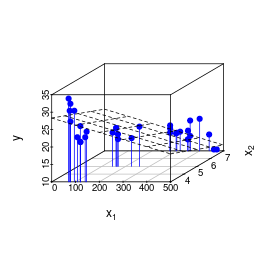
\includegraphics[width=0.8\textwidth, trim=0 40 0 0, clip]{
    figure/lm_3d.png} \\
    \tiny{Linear regression hyperplane}
  \end{center}
\end{minipage}
\begin{minipage}[b]{0.24\textwidth}
  \begin{center}
     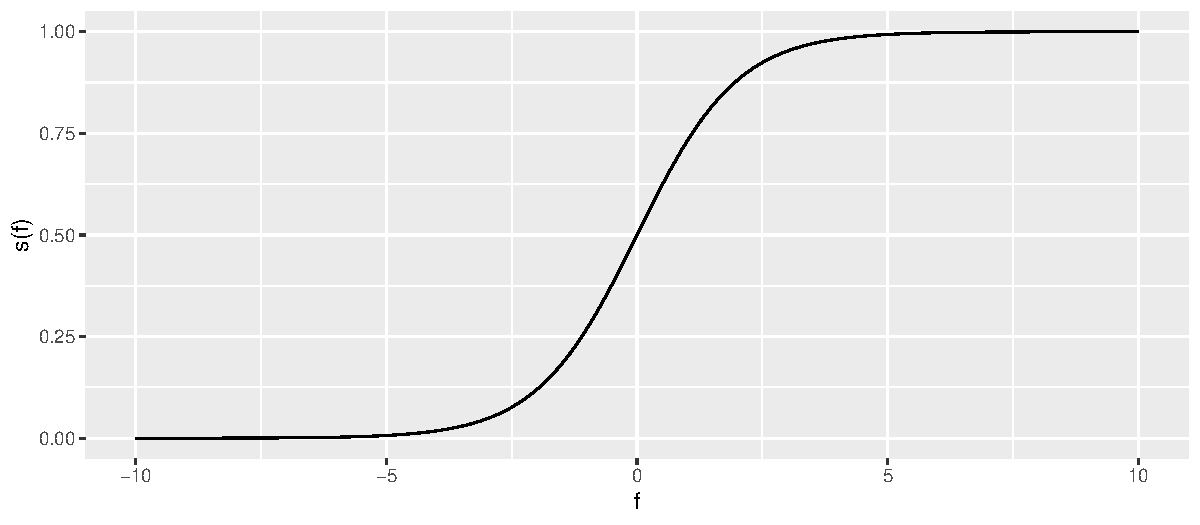
\includegraphics[width=0.7\textwidth, trim=0 40 0 0, clip]{../slides/supervised-classification/figure/reg_class_log_1}\\
    \tiny{Logistic sigmoid function}
  \end{center}
\end{minipage}
\begin{minipage}[b]{0.24\textwidth}
  \begin{center}
    % 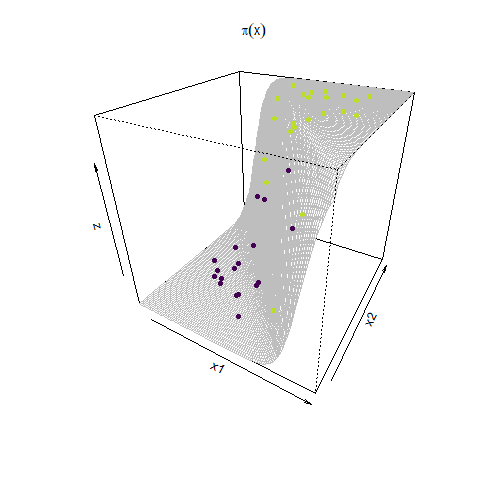
\includegraphics[width=0.7\textwidth, trim=0 40 0 0, clip]{
    % ../slides/supervised-classification/figure_man/logreg-2vars-surface}\\
    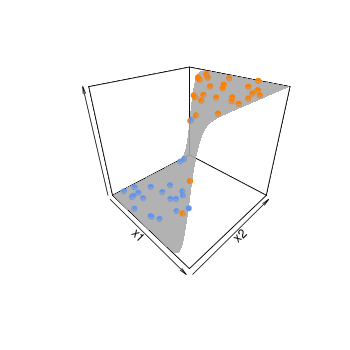
\includegraphics[width=0.65\textwidth, trim=30 50 0 0, clip]{
    figure/logreg_3d}\\
    \tiny{Logistic function for bivariate input and loss-minimal $\thetab$}
  \end{center}
\end{minipage}
\begin{minipage}[b]{0.24\textwidth}
  \begin{center}
    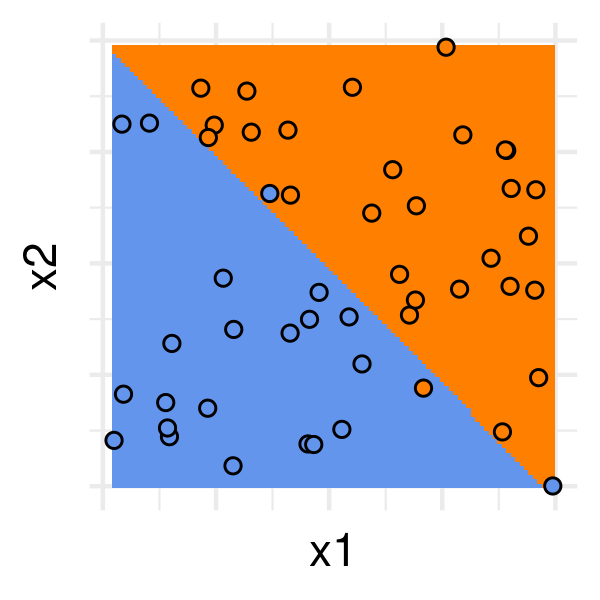
\includegraphics[width=0.5\textwidth]{figure/logreg_2d}\\
    % 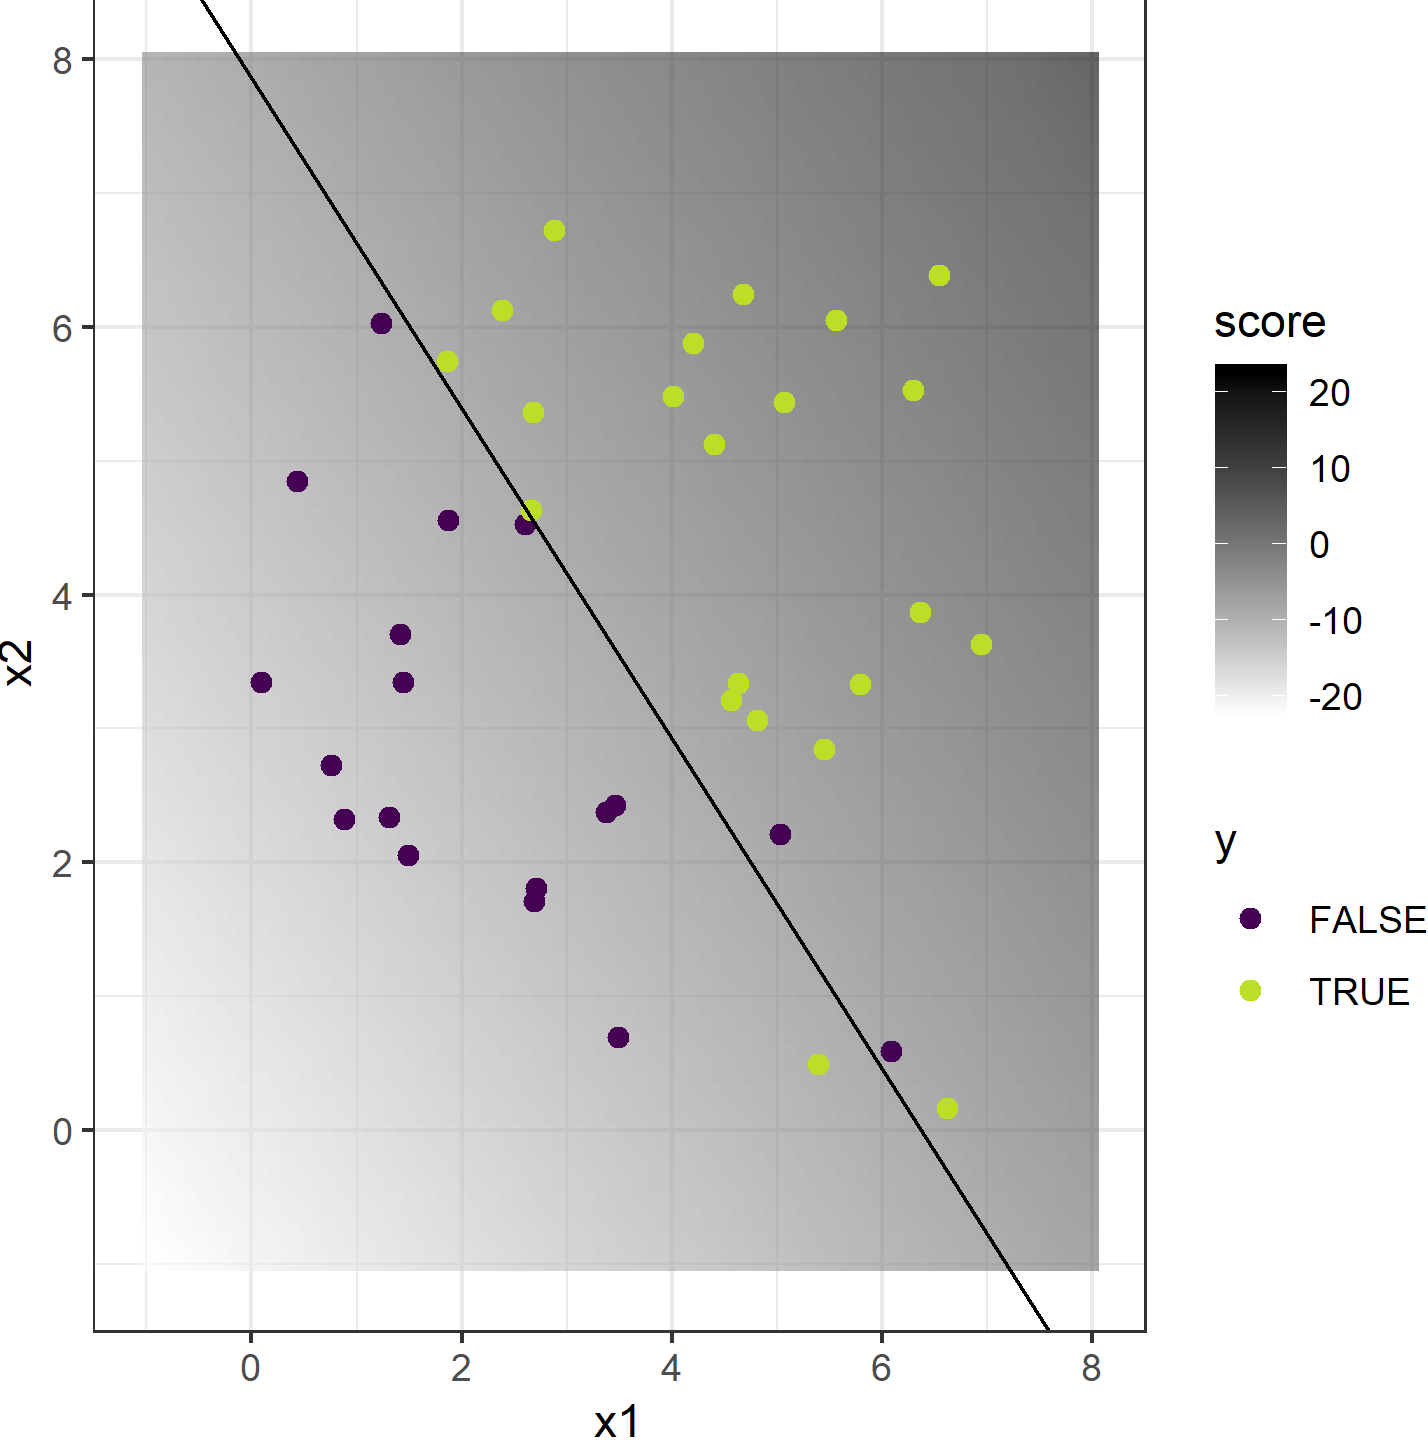
\includegraphics[width=0.6\textwidth]{
    % ../slides/supervised-classification/figure_man/logreg-2vars-data} \\
    \tiny{Corresponding separating hyperplane}
\end{center}
\end{minipage}

\framebreak

\highlight{Loss functions}

\begin{itemize}
  \item \textbf{Lin. Regr.}:
  \begin{itemize}
    
    \item Typically, based on \textbf{quadratic} loss (OLS estimation): 
    $$L\left(y, f\right) = \left(y - f \right)^2$$ %~~
    %$\Rightarrow$ OLS estimation
    % \item Alternatives: e.g., \textbf{absolute} or \textbf{Huber} loss (both 
    % improving robustness)
  \end{itemize}
  \item \textbf{Log. Regr.}: Based on \textbf{bernoulli / log / cross-entropy} loss ~ 
  %$\Rightarrow \risket = \sumin -\yi \log \left(\pixii\right) - (1 - \yi) \log \left(1 - \pixii \right)$
  \begin{itemize}
      \item Loss based on scores
      \begin{eqnarray*}
    L\left(y, f\right) &=& \ln\left(1+\exp\left(-y \cdot f\right)\right) \quad \text{for } y \in \setmp\\
    L\left(y, f\right) &=& - y \cdot f + \log\left(1 + \exp\left(f\right)\right) \quad \text{for } y \in \setzo 
    \end{eqnarray*}
    \item Loss based on probabilities:
      \begin{eqnarray*}
    L\left(y, \pi\right) &=& \ln\left(1+\exp\left(-y \cdot \log \left(\pi\right)\right)\right) \quad \text{for } y \in \setmp\\
    L\left(y, \pi\right) &=& -y \log \left(\pi\right) - (1 - y) \log \left(1 - \pi \right)  \quad \text{for } y \in \setzo 
    \end{eqnarray*}
  \end{itemize}
\end{itemize}

\framebreak

\medskip

\highlight{Optimization} 

\begin{itemize}
    \item Minimization of the empirical risk
    \item For \textbf{OLS}: analytical solution $\thetabh = \olsest$
    \item For other loss functions: 
    \begin{itemize}
        \item \textbf{Log. Regr.}: Convex problem, solvable via second-order optimization methods (e.g. BFGS)
        \item \textbf{Else}: Numerical optimization 
    \end{itemize}
    
\end{itemize}

\medskip

% \highlight{Hyperparameters} ~~ None

%\medskip

\highlight{Multi-class extension of logistic regression}

\begin{itemize}
  \item Estimate \textbf{class-wise} scoring functions:
  $\Rightarrow \pi: \Xspace \rightarrow \unitint^g, ~
  \pix = (\pikx[1], \dots, \pikx[g]), ~\sumkg \pikx = 1$
  \item Achieved through \textbf{softmax} transformation: 
  $\pikxt = \exp(\thetab_k^\top \xv) \big/ \sum_{j=1}^g \exp(\thetab_j^\top 
  \xv)  $
  \item Multi-class log-loss: $\Lpixy = - \sumkg \I_{\{y = k\}} \log(\pikx)$
  \item Predict class with maximum score (or use thresholding variant)
\end{itemize}

% \highlight{Runtime behavior} ~~ $\mathcal{O}(p^2 \cdot n + p^3)$ for $n$ 
% observations and $p$ features

\end{vbframe}


% ------------------------------------------------------------------------------

\begin{frame}{Generalized Linear Models -- regularization}

\highlight{General idea}

\begin{itemize}
  \item Unregularized LM: risk of \textbf{overfitting} in high-dimensional 
  space with only few observations
  %\item \textbf{Goal}: find compromise between model fit and generalization by adding \textbf{penalty term}
  \item \textbf{Goal}: avoidance of overfitting by adding \textbf{penalty term}
%  \item Regularization ubiquitous in ML, with similar techniques
\end{itemize}

%\medskip

% \highlight{Hypothesis space} ~~\\
% $\Hspace = \left\{f: \Xspace \to \R ~|~\fx = \phi(\thetab^\top \xv)\right\}$, 
% where $\phi(\cdot)$ is a transformation function.


%$\Hspace = \{ \theta_0 + \thx\ |\ (\theta_0, \thetab) \in \R^{p+1} \} $

\medskip
\begin{columns}[T, totalwidth=\textwidth]
    \begin{column}{0.55\textwidth}
        
\highlight{Regularized empirical risk}

\begin{itemize}
  \item Empirical risk function \textbf{plus complexity penalty} 
  $J(\thetab)$, controlled by shrinkage parameter $\lambda > 0$:
  $\riskrt := \risket + \lambda \cdot J(\thetab)$
  %\item Popular regularizers
  %\begin{itemize} 
    \item \textbf{Ridge} regression: L2 penalty $J(\thetab) = \|\thetab\|_2^2 $
    \item \textbf{LASSO} regression: L1 penalty $J(\thetab) = \|\thetab\|_1 $
  %\end{itemize}
\end{itemize}

\medskip

\highlight{Optimization under regularization}
\begin{itemize}
  \item \textbf{Ridge}: analytically with 
  $\thetabh_{\text{Ridge}} = (\Xmat^\top \Xmat  + \lambda \id)^{-1} \Xmat^\top 
  \yv$
  \item \textbf{LASSO}: numerically with, e.g., (sub-)gradient descent
\end{itemize}



    \end{column}
        \begin{column}{0.45\textwidth}
          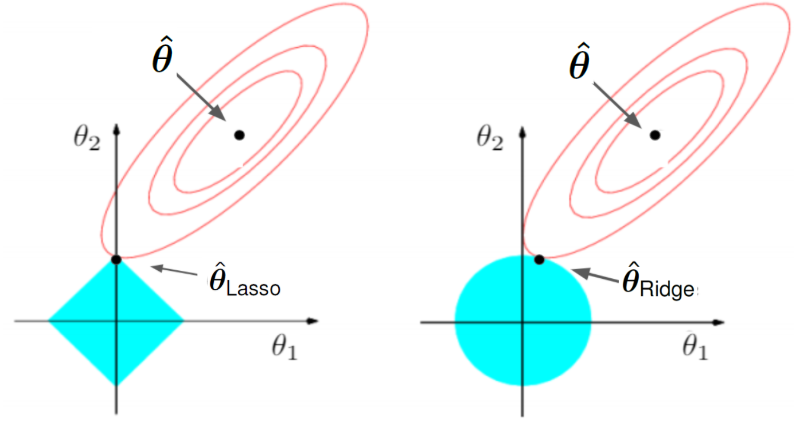
\includegraphics[width=\textwidth]{figure/l1_l2_hat.png}
    \end{column}
\end{columns}

\medskip
\highlight{Choice of regularization parameter}

\begin{itemize}
  \item Standard hyperparameter optimization problem
  \item E.g., choose $\lambda$ with minimum mean cross-validated error 
  %(default in R package \texttt{glmnet})
\end{itemize}
\end{frame}

% ------------------------------------------------------------------------------

\begin{frame}{Generalized Linear Models -- regularization}

  \begin{columns}[T, totalwidth=\textwidth]
  \begin{column}{0.62\textwidth}

\highlight{Ridge vs. LASSO} 

\begin{itemize}
  \item \textbf{Ridge}
  \begin{itemize} 
    \item Global shrinkage $\Rightarrow$ overall smaller but still dense $\thetab$
    \item Applicable with large number of influential features, handling 
    correlated variables by shrinking their coefficients by equal amount
  \end{itemize}
  \item \textbf{LASSO}
  \begin{itemize} 
    \item Actual variable selection by shrinking coefficients for irrelevant 
    features all the way to zero
    \item Suitable for sparse problems, ineffective with correlated 
    features (randomly selecting one)
  \end{itemize}  
  \item Neither overall better $\Rightarrow$ compromise: \textbf{elastic net}
  \begin{itemize} 
    \item Weighted combination of Ridge and LASSO
    \item Introducing additional penalization coefficient: %$\riskrt = \risket + \lambda_1 \cdot \|\thetab\|_1 + \lambda_2 \cdot \|\thetab\|_2^2$\\
    $\riskrt = \risket 
    + \lambda \cdot P_{\alpha}(\thetab)$, with\\
    $P_{\alpha}(\thetab) = [\alpha \cdot \|\thetab\|_1 + (1 - \alpha) \cdot \frac{1}{2} \cdot \|\thetab\|_2^2]$
  \end{itemize}  
\end{itemize}

\end{column}

\begin{column}{0.38\textwidth}
\tiny
\centering
\begin{columns}[T, totalwidth=\textwidth]
\begin{column}{0.5\textwidth}
\tiny
\begin{center}
\textbf{Ridge} performs better for correlated features: \\ 
\medskip
$\boldsymbol{\beta}=(\underbrace{2,\ldots,2}_{5},\underbrace{0,\ldots,0}_{5})$\\
$ \operatorname{cor}(\Xmat_{i},\Xmat_{j})=0.8^{|i-j|}, \forall i, j$
  \end{center}
\end{column}
\begin{column}{0.5\textwidth} \tiny

\begin{center}
\textbf{Lasso} performs better for uncorrelated features: \\
\medskip
$\boldsymbol{\beta}=(2, 2, 2,\underbrace{0,\ldots,0}_{7})$ \\
$\operatorname{cor}(\Xmat_{i},\Xmat_{j})= 0, \forall i \neq j$
\end{center}
\end{column}
\end{columns}



          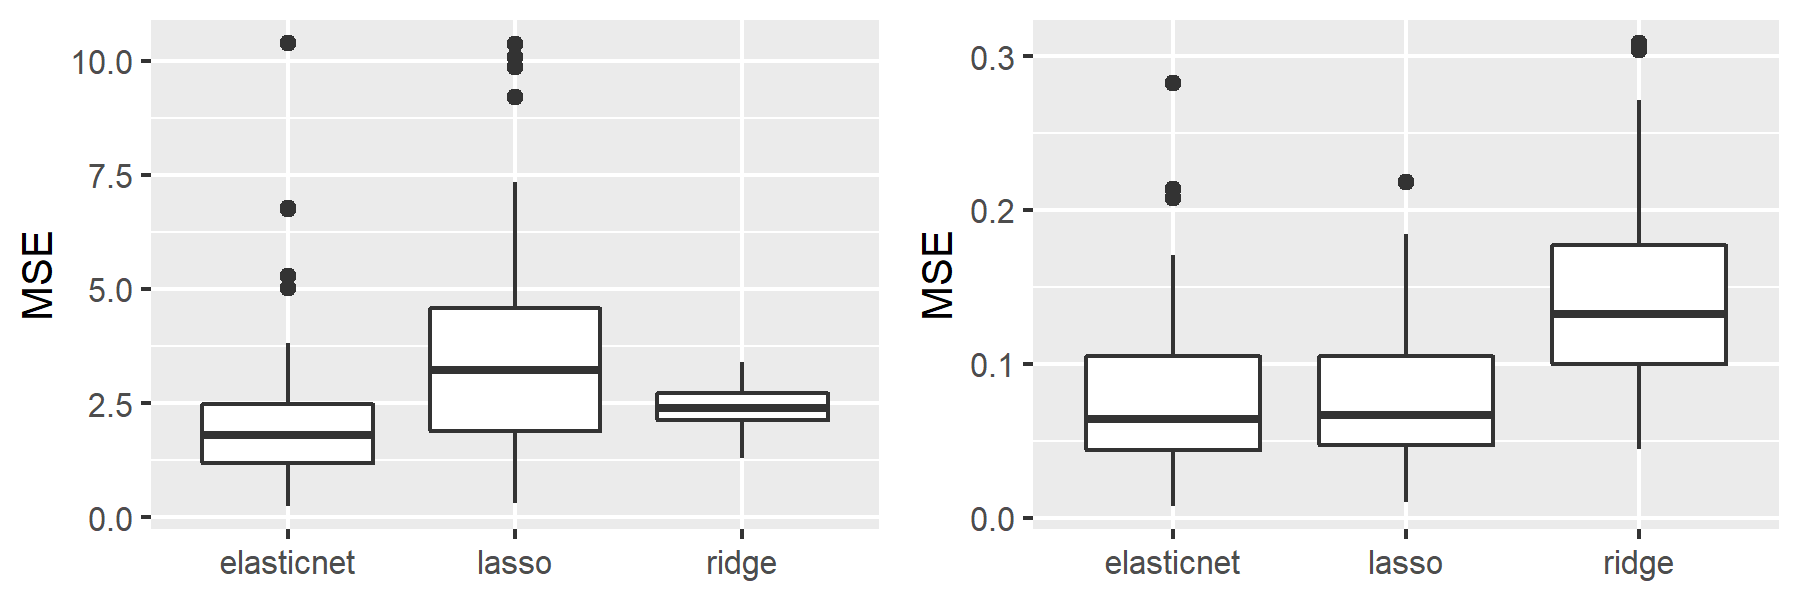
\includegraphics[width=\textwidth]{figure/enet_lasso_ridge_mse.png}
          
          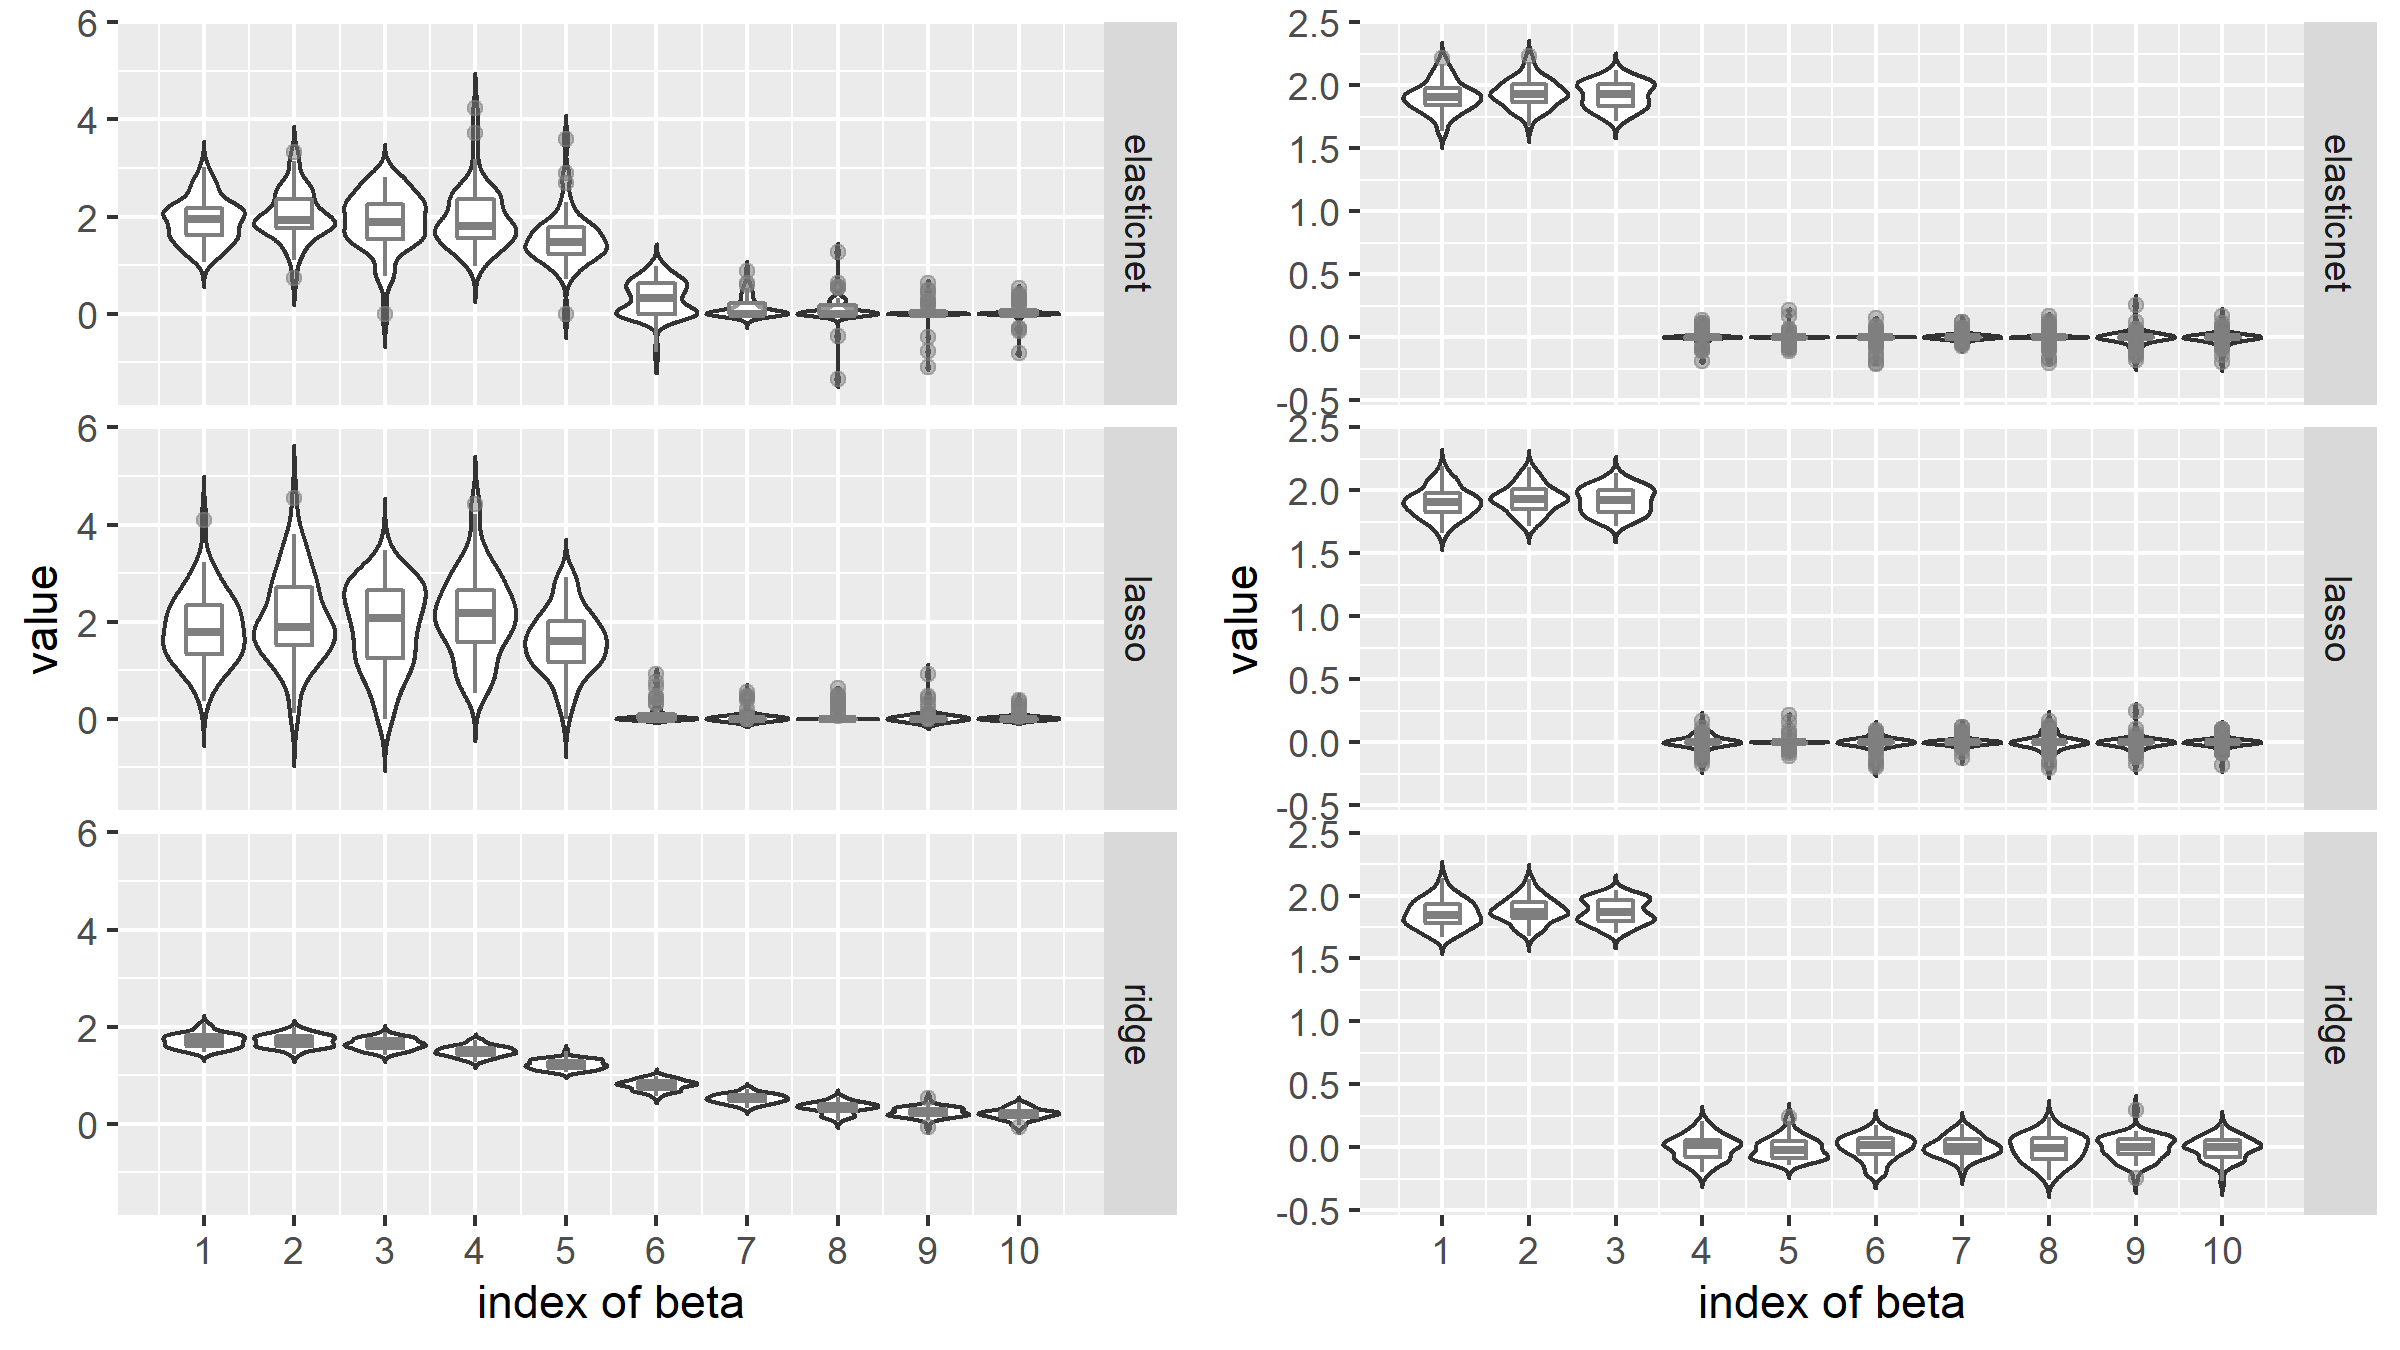
\includegraphics[width=\textwidth]{figure/enet_tradeoff.png}
\end{column}

\end{columns}

\end{frame}

% ------------------------------------------------------------------------------

\begin{frame}{Generalized Linear Models -- Implementation}

\highlight{Implementation}

\begin{itemize}
  \item \textbf{R:}
  \begin{itemize}
    \item \textbf{Unregularized:} \texttt{mlr3} learner \texttt{LearnerRegrLM}, 
    calling \texttt{stats::lm()} / \texttt{mlr3} learner 
    \texttt{LearnerClassifLogReg}, calling \texttt{stats::glm()}
    \item \textbf{Regularized / ElasticNet:} \texttt{mlr3} learners 
    \texttt{LearnerClassifGlmnet} / 
    \texttt{LearnerRegrGlmnet}, calling \texttt{glmnet::glmnet()}
    \item For \textbf{large classification} data: \texttt{mlr3} learner     
    \texttt{LearnerClassifLiblineaR}, calling \texttt{LiblineaR::LiblineaR()} uses fast coordinate descent
  \end{itemize}
  \item \textbf{Python:} From package \texttt{sklearn.linear\_model} 
  \begin{itemize}
    \item \textbf{Unregularized:}\\ 
    - \texttt{LinearRegression()}\\
    - \texttt{LogisticRegression(penalty = None)}
    \item \textbf{Regularized:}\\
    - \textit{Linear regression:} \texttt{Lasso(),Ridge(),ElasticNet()} \\
    - \textit{Logistic regression:} \texttt{LogisticRegression(penalty = \{‘l1’, ‘l2’, ‘elasticnet’\})}
    \item Package for advanced \textbf{statistical} models: \texttt{statsmodels.api} 
  \end{itemize}
\end{itemize}

%% WOULD DELTETE THIS!
%  \highlight{\textcolor{blue}{Check assumptions??} }\\
% Linear models are effective if the following assumptions are fulfilled:
%  \begin{itemize}
%   \item \textbf{linearity}: The expected response is a linear combination of the features.
%   \item \textbf{homoscedasticity}: The variance of residuals is equal for all features.
%   \item \textbf{independence}: All observations are independent of each other.
%   \item \textbf{normality}: Y is normally distributed for any fixed value of the features
% \end{itemize}

\end{frame}


% ------------------------------------------------------------------------------

\begin{frame}{Generalized Linear Models -- Pros \& Cons}



\begin{columns}[onlytextwidth]
  \begin{column}{0.5\textwidth}
    \highlight{Advantages}
    
    \begin{procon}
      \setlength{\itemsep}{1pt}
      \setlength{\parskip}{1pt}
      \positem \textbf{Simple and fast} implementation
      \positem \textbf{Analytical} solution for L2 loss
      %\positem \textbf{Cheap} computation
      \positem Applicable for any \textbf{dataset size}, as long as number of 
      observations $\gg$ number of features
      \positem Flexibility \textbf{beyond linearity} with polynomials, 
      trigonometric transformations, interaction terms etc.
      \positem Intuitive \textbf{interpretability} via feature effects
      % \item fits \textbf{linearly} separable data sets very well
      \positem Statistical hypothesis \textbf{tests} for effects available
    \end{procon}
  \end{column}

  \begin{column}{0.5\textwidth}
    \highlight{Disadvantages}
    
    \begin{itemize}
      \negitem \textbf{Nonlinearity} of many real-world problems
      \negitem Further restrictive \textbf{assumptions}: linearly independent 
      features, homoskedastic residuals, normality of conditional response 
      %\textcolor{blue}{actually relevant in ML?}
      \negitem \textbf{Sensitivity} w.r.t. outliers and noisy data (especially 
      with L2 loss)
      \negitem Also a LM can \textbf{overfit} (e.g., many features and few observations) 
      \negitem Feature \textbf{interactions} must be handcrafted\\
      $\rightarrow$ practically infeasible for higher orders
      %\negitem No handling of \textbf{missing} data
    \end{itemize}
  \end{column}
\end{columns}

\end{frame}